


\begin{frame}{Outline}
  \begin{itemize}
  \item \textcolor{gray}{Background: Core Model and Implementation}
    \air
  \item \textcolor{gray}{Work 1: Controlling  Generation  }
    \air

  \item \textcolor{gray}{Work 2: Controlling Attention (\textit{Variational Attention})}
    \air


  \item \textbf{Challenges: Text Generation and Deep Learning}
  \end{itemize}

\end{frame}



% \begin{frame}{Research Approach}

%   \begin{center}
%    Machine learning methods to push improvements in natural language.
%     \air
%     \[ \Updownarrow \]
%     Natural language processing for motivating new methods in machine learning.
%   \end{center}
% \end{frame}



\begin{frame}{Reasoning Systems for Long-Form Generation}
  \begin{center}
    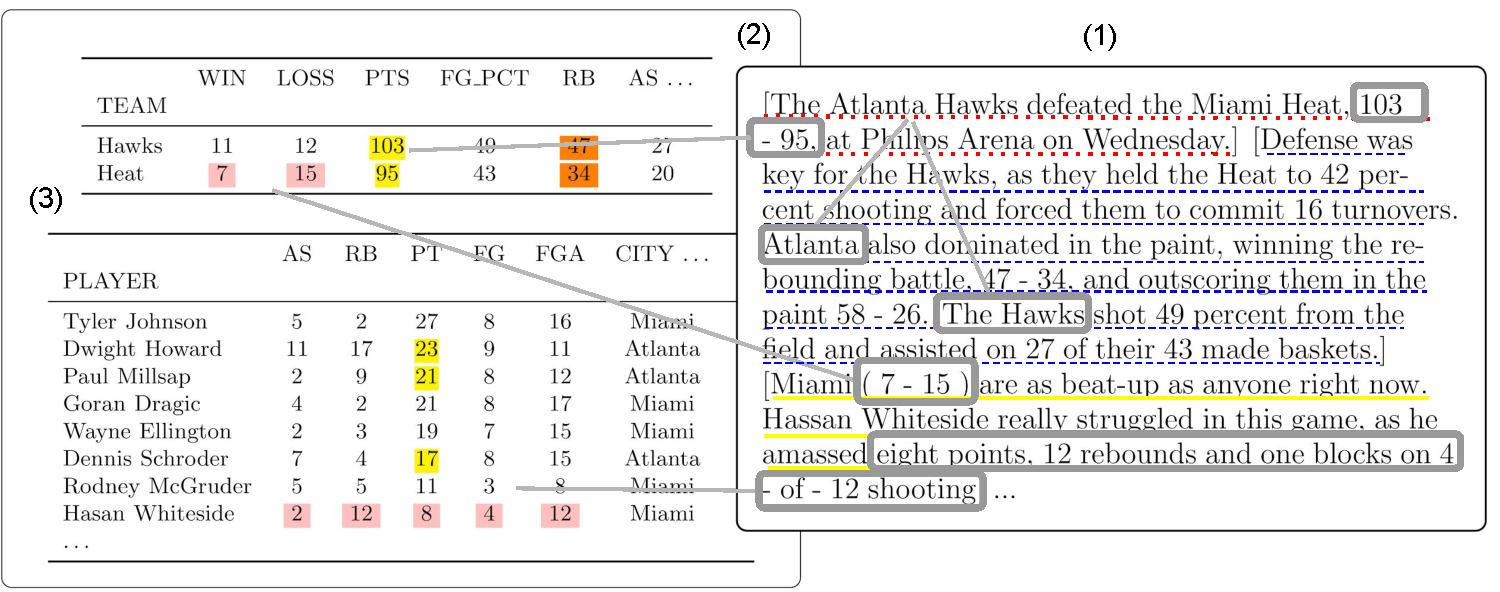
\includegraphics[width=0.85\linewidth]{basketball}
  \end{center}
\end{frame}


% \begin{frame}{Three Challenge in Text Generation}
%   \begin{enumerate}
%   \item Long-Form Generation with High-Level Reasoning
%     \air
%   \item Compact and Efficient Generation
%     \air
%   \item Latent-Variable Modeling for NLP
%   \end{enumerate}
% \end{frame}

% \begin{frame}{Future Work}

%   \begin{center}
%   \begin{tikzpicture}
%     \node[rounded corners, draw] (ana) at (-15mm, 15mm) {Analysis};
%     \node[rounded corners, draw] (meth) at (0mm, 30mm) {\ Methods\phantom{p}};
%     \node[rounded corners, draw] (app) at (25mm, 30mm) {Applications};
%     \node[rounded corners, draw] (und) at (35mm, 15mm) {Understanding};
%     \node[rounded corners, draw] (dep) at (25mm, 0mm){Deployment};
%     \node[rounded corners, draw] (imp) at (0, 0) {Implement};
%     \draw (ana) -- (meth) --(app) -- (und) -- (dep) -- (imp) -- (ana);
%   \end{tikzpicture}
%   \end{center}
% \end{frame}



% \begin{frame}{1) Long-Form Generation with Explicit Reasoning}
%   \begin{center}
%     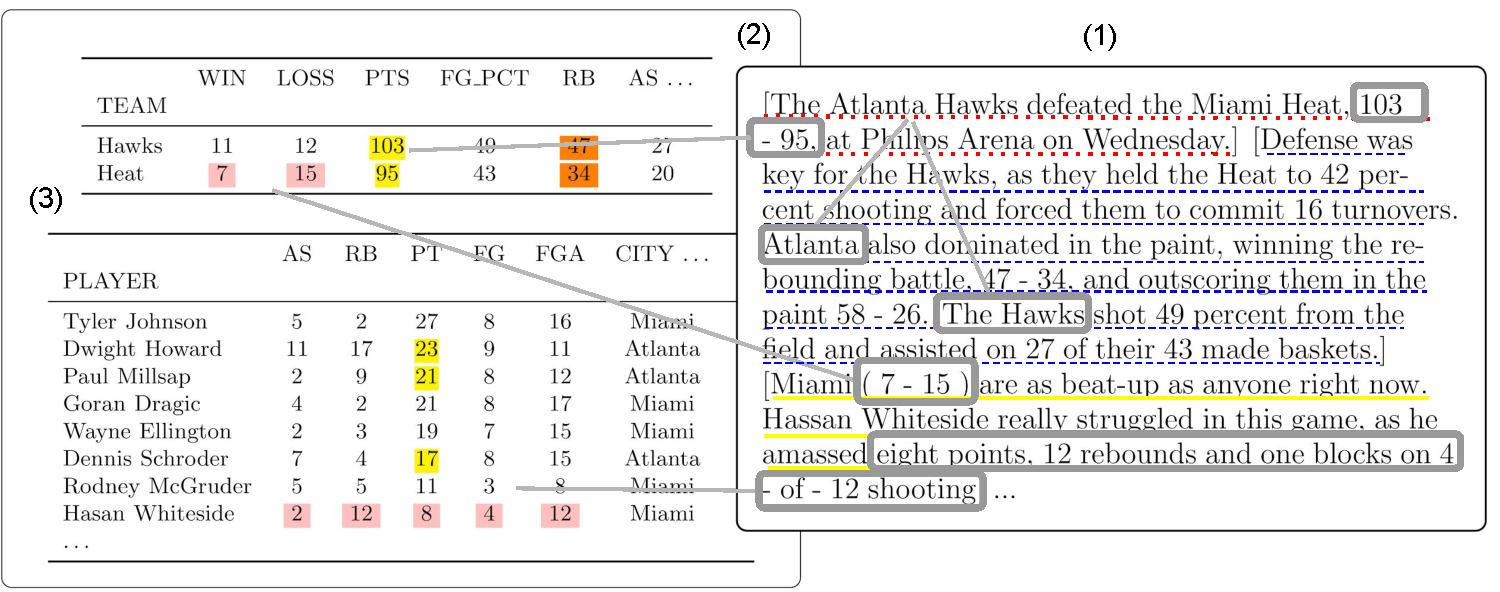
\includegraphics[width=0.85\linewidth]{basketball}
%   \end{center}
%   % \begin{enumerate}
%   % \item Discourse-aware structure in generation
%   % \item Explicit Linking and coreference
%   % \item Aggregation of factual information before generation
%   % \end{enumerate}
% \end{frame}

% \begin{frame}{2) Controllable Interactive ML Systems}
%   \research{w/ IBM}
%   \begin{center}
%     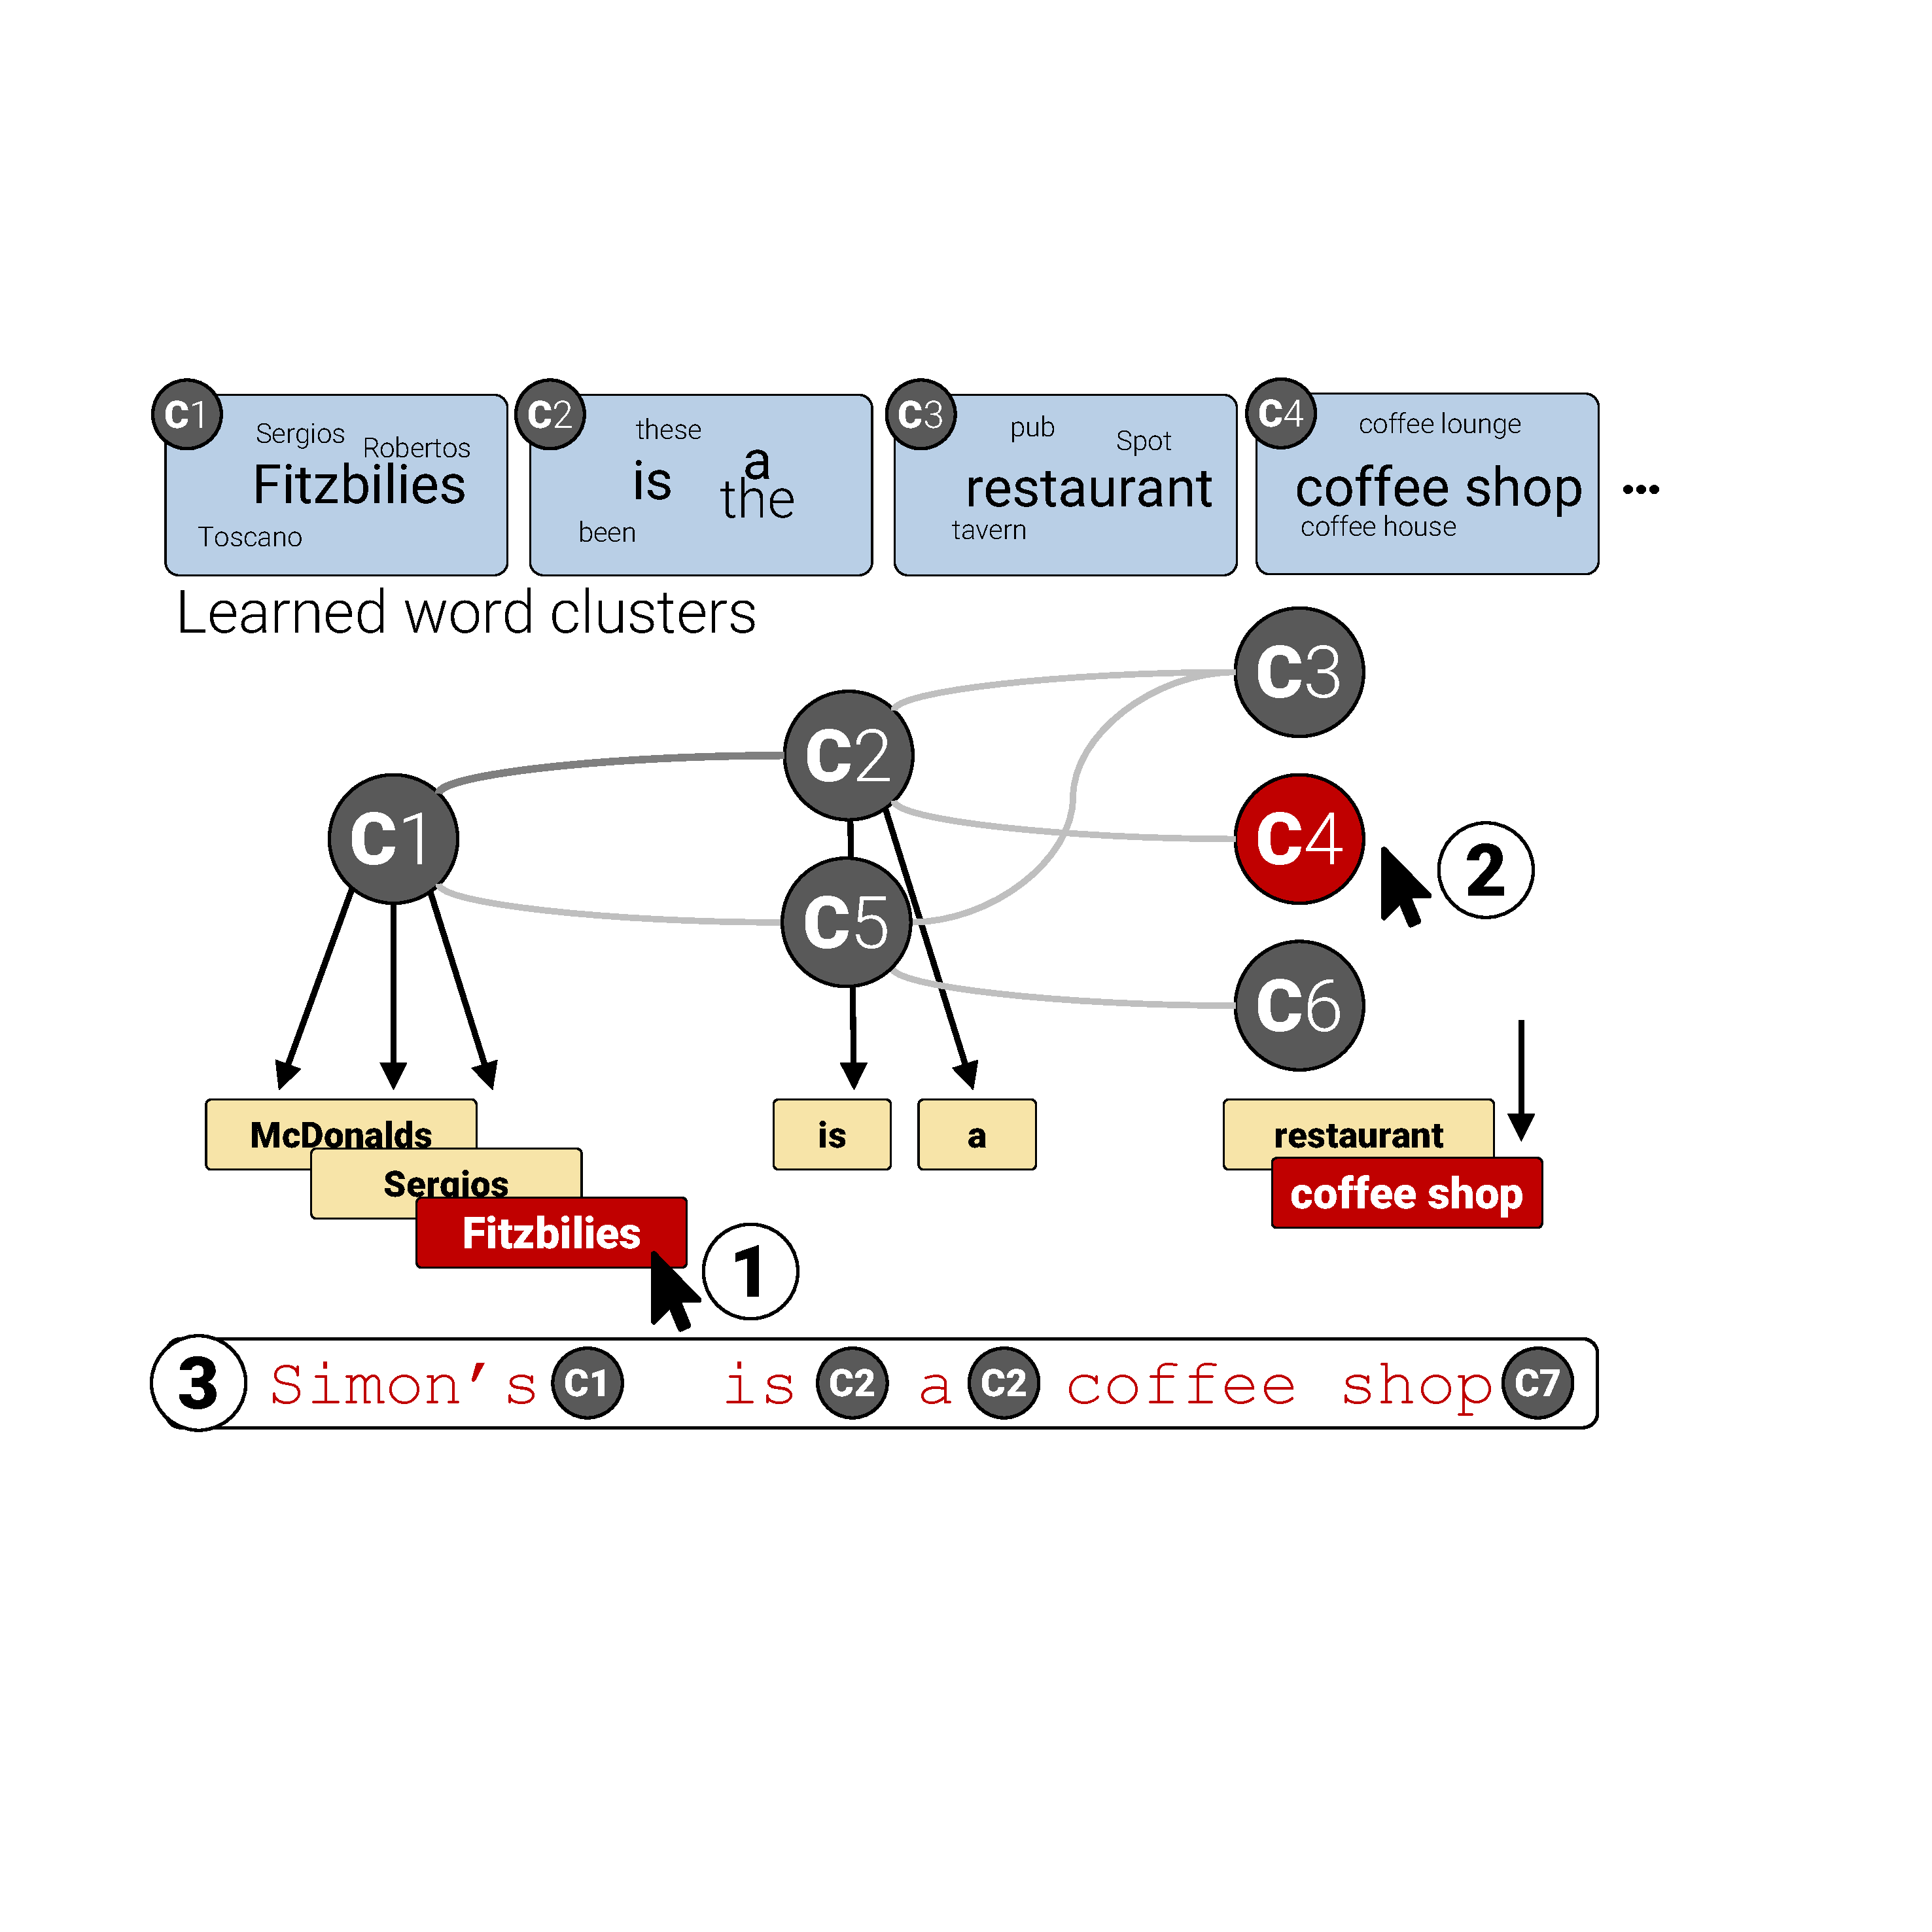
\includegraphics[width=0.7\textwidth]{DecoderVis}
%   \end{center}
% \end{frame}


\begin{frame}{Controllable Deep Learning for Translation}
  \research{w/ IBM}
  \begin{center}
    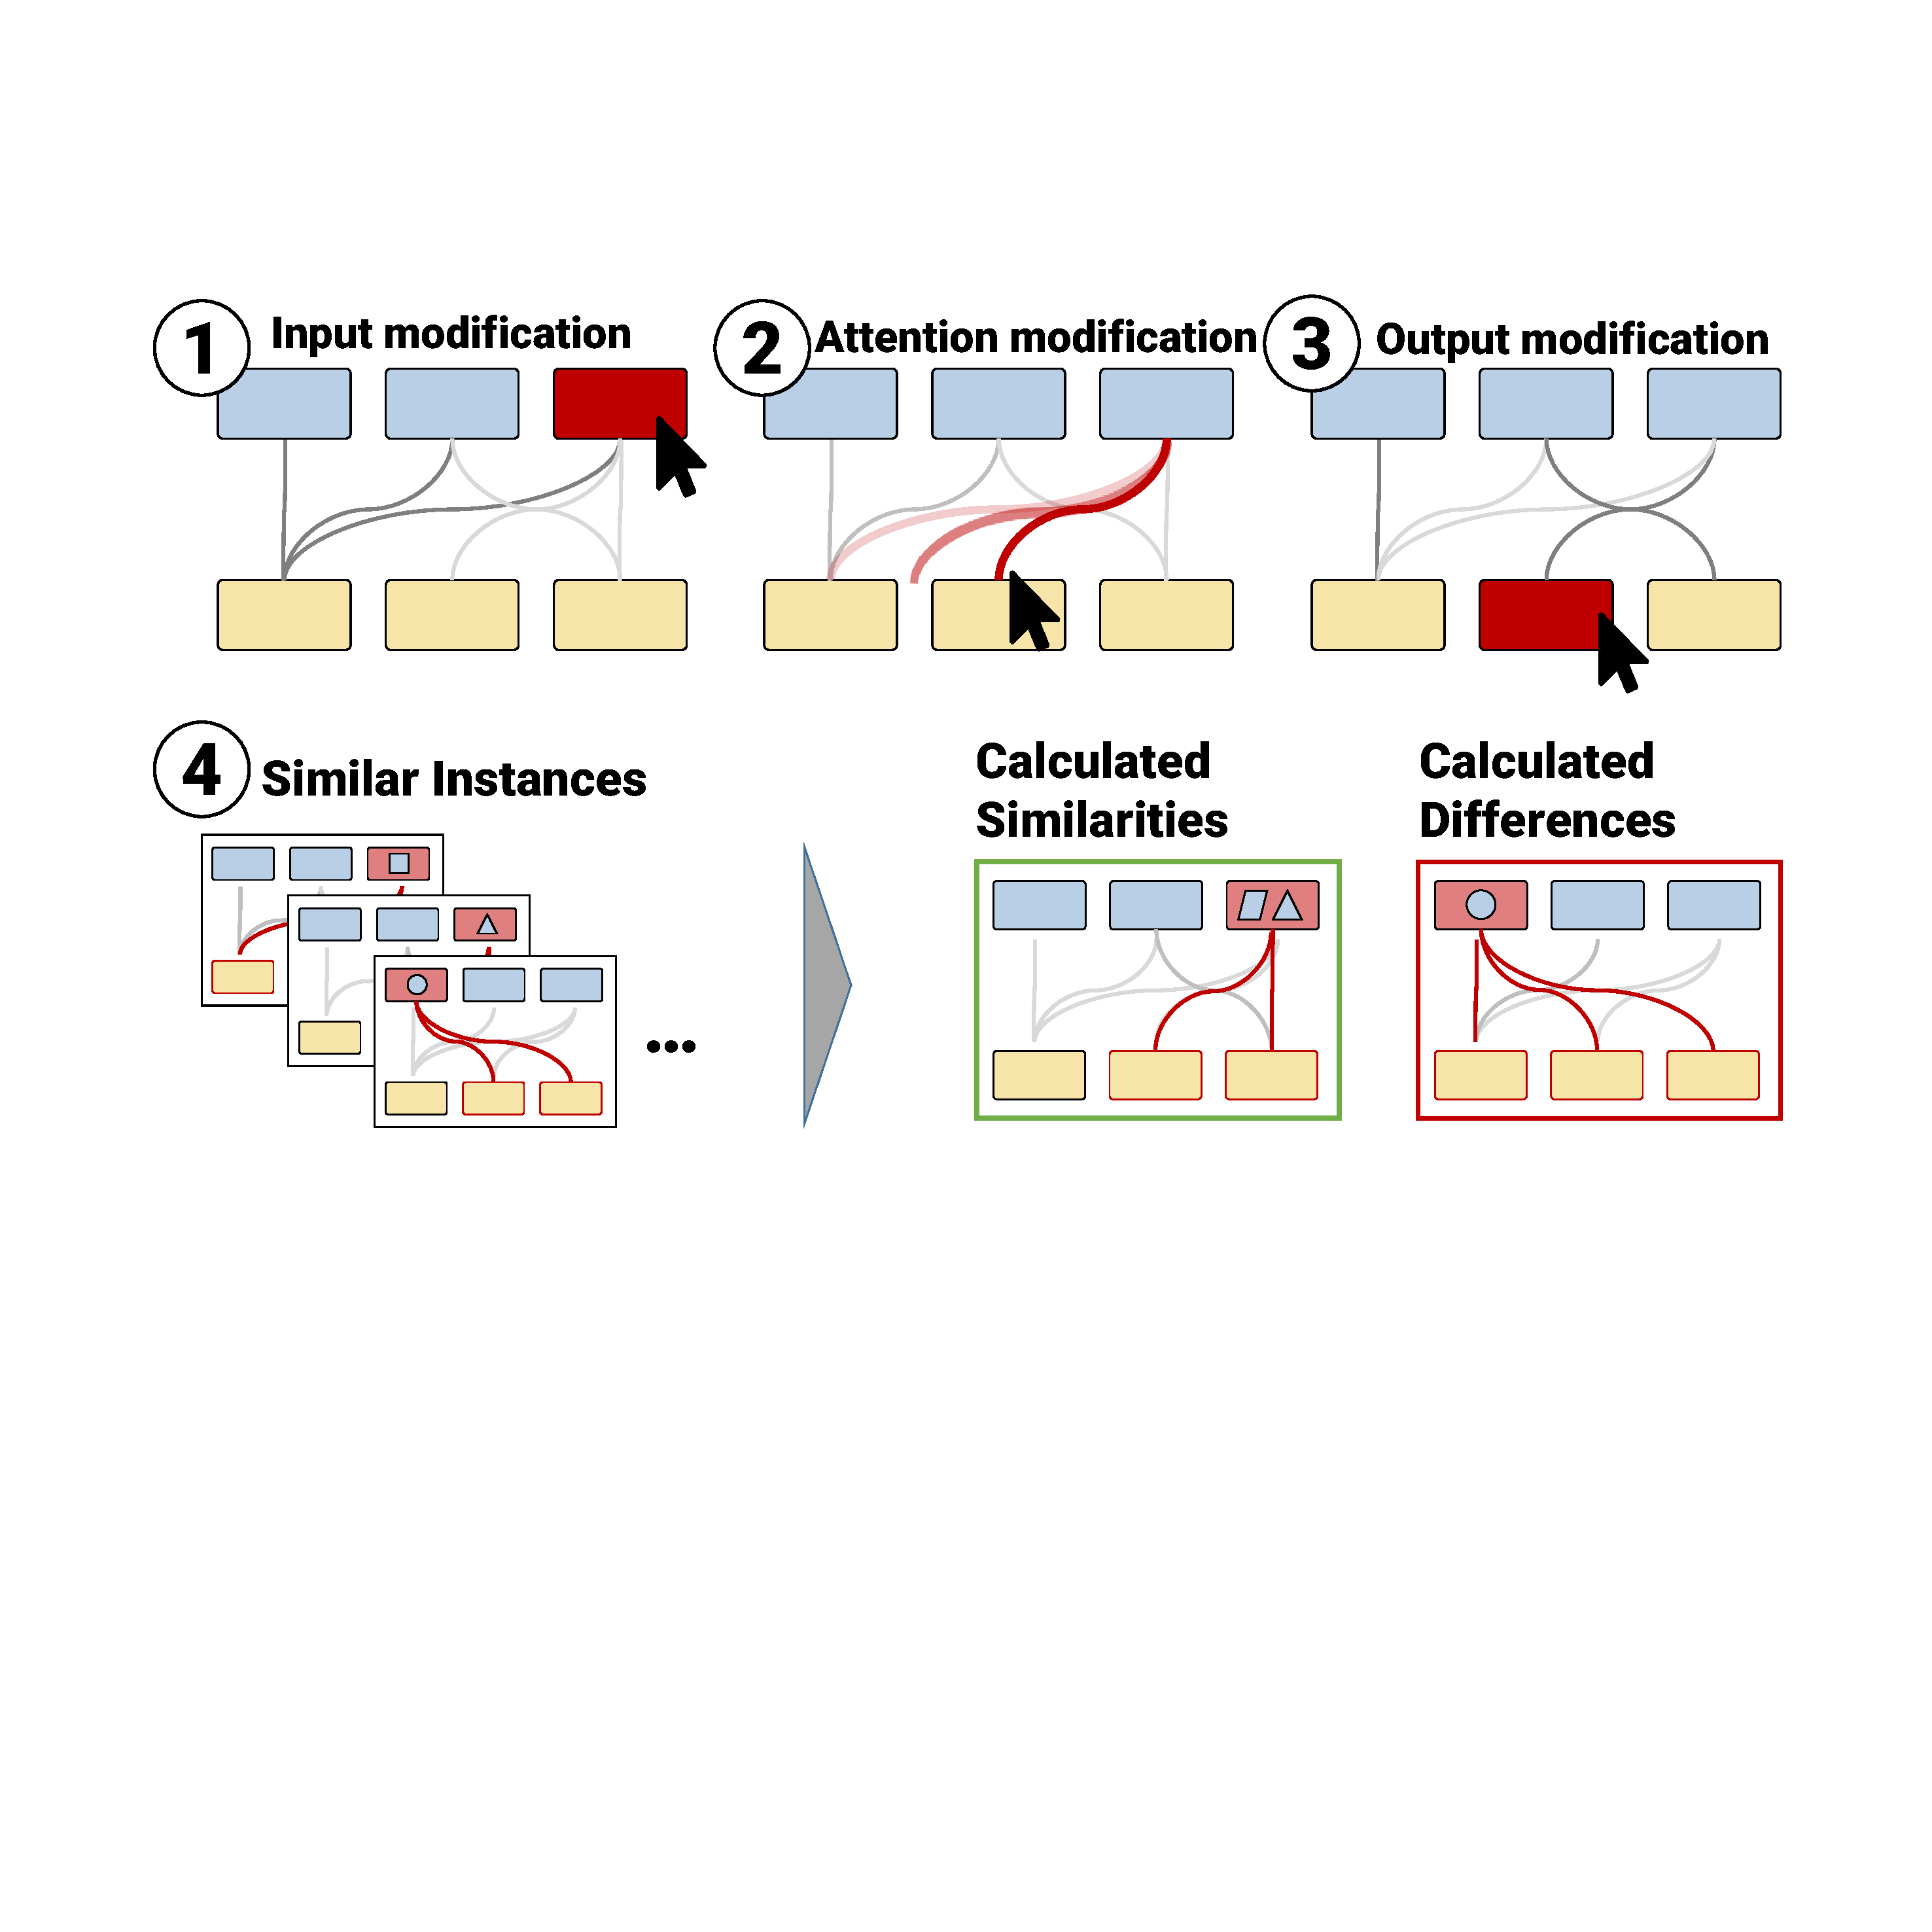
\includegraphics[width=0.8\textwidth]{AttentionVIS}
  \end{center}
\end{frame}

\begin{frame}{Prob. Programs for Language Understanding}
\research{w/ Uber}

\begin{center}

\includegraphics[width=3cm]{pyro} \hspace{2cm} 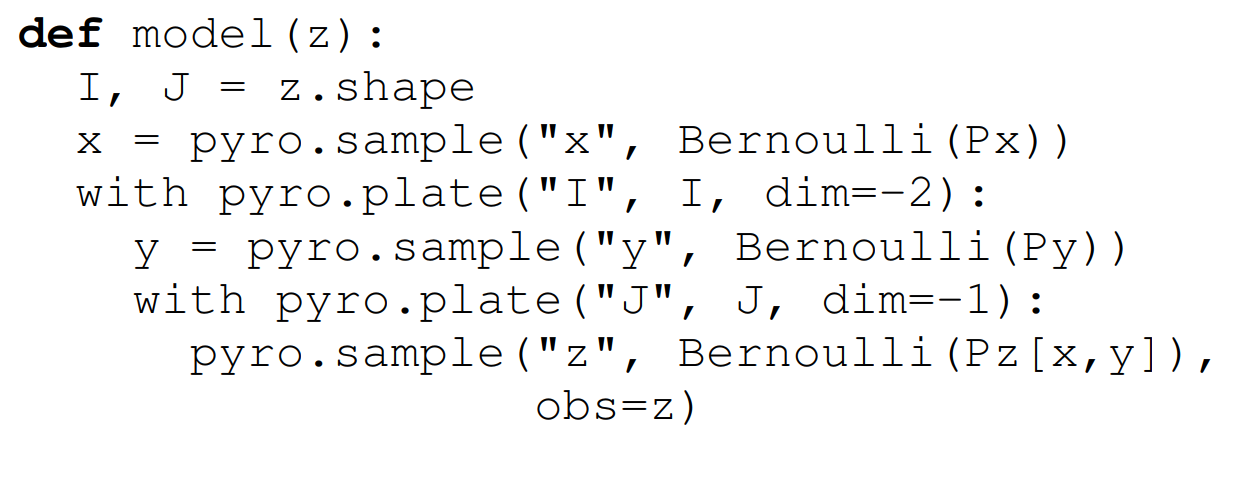
\includegraphics[width=5cm]{pyro2}

\air
  \begin{tikzpicture}
\node[latent] (Y) {$y$};
\node[factor, xshift=1.25cm] (FYS) {$F$};
\node[latent, xshift=2.5cm](S) {$z$};
\node[factor, xshift=3.75cm](FS) {$G$};
\node[xshift=1.25cm, yshift=-0.5cm]() {$T$};
\node[obs, xshift=5cm](X) {$\mathbf{x}$};
\node[obs, xshift=2.5cm, yshift=1.3cm] (A) {$a$};
\node[obs, xshift=2.5cm, yshift=-1.45cm] (L) {$l$};


\plate [inner sep=0.1cm, xshift=0cm, yshift=0.0cm] {t} {(FS)(S)(FYS)} {};
\plate [inner xsep= 0.3cm, inner ysep= 0.2cm, xshift=-0.1cm, yshift=-0.1cm] {a} {(Y)(FYS)(S)(A)(FS)} {};
\plate [inner xsep= 0.3cm, inner ysep= 0.1cm, xshift=0.1cm, yshift=0.2cm] {l} {(Y)(FYS)(S)(L)(FS)} {};
\node[caption, below left=-0.1cm and -0.3cm of a-wrap.north west] {$|\cal{A}|$};
\node[caption, below left=-0.5cm and -0.4cm of l-wrap.south east] {$|\cal{L}|$};

\draw (Y) -- (FYS);
\draw (X) -- (FS);
\draw[-] (X) to [bend left=25] (FYS);
\draw (FYS) -- (S);
\draw (S) -- (FS);
\draw (FS) -- (A);
\draw (FS) -- (L);
\draw[-] (FYS) to [] (A);
\draw[-] (FYS) to [] (L);
\end{tikzpicture}

\end{center}
\end{frame}


% \begin{frame}{Hardware for Deep Learning}
% \research{w/ ARM}
% \begin{center}
%   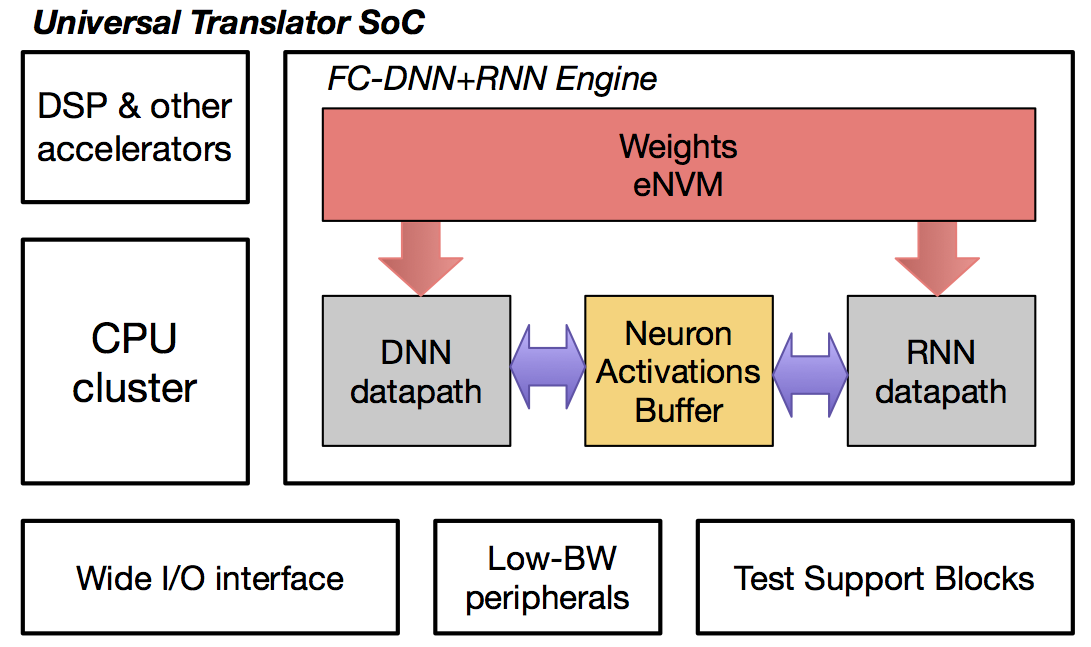
\includegraphics[height=0.6\textheight]{testchip}
% \end{center}
% \end{frame}



% \begin{frame}{Learning Neural Reasoning-Based Models}
%   \begin{center}
%     \movie[width=\textwidth, repeat, height=0.85\textheight, width=\textwidth, poster, showcontrols]{Temporary}{videos/latnm.mp4}
%   \end{center}
% \end{frame}


\begin{frame}{Harvard NLP}
  \begin{center}
  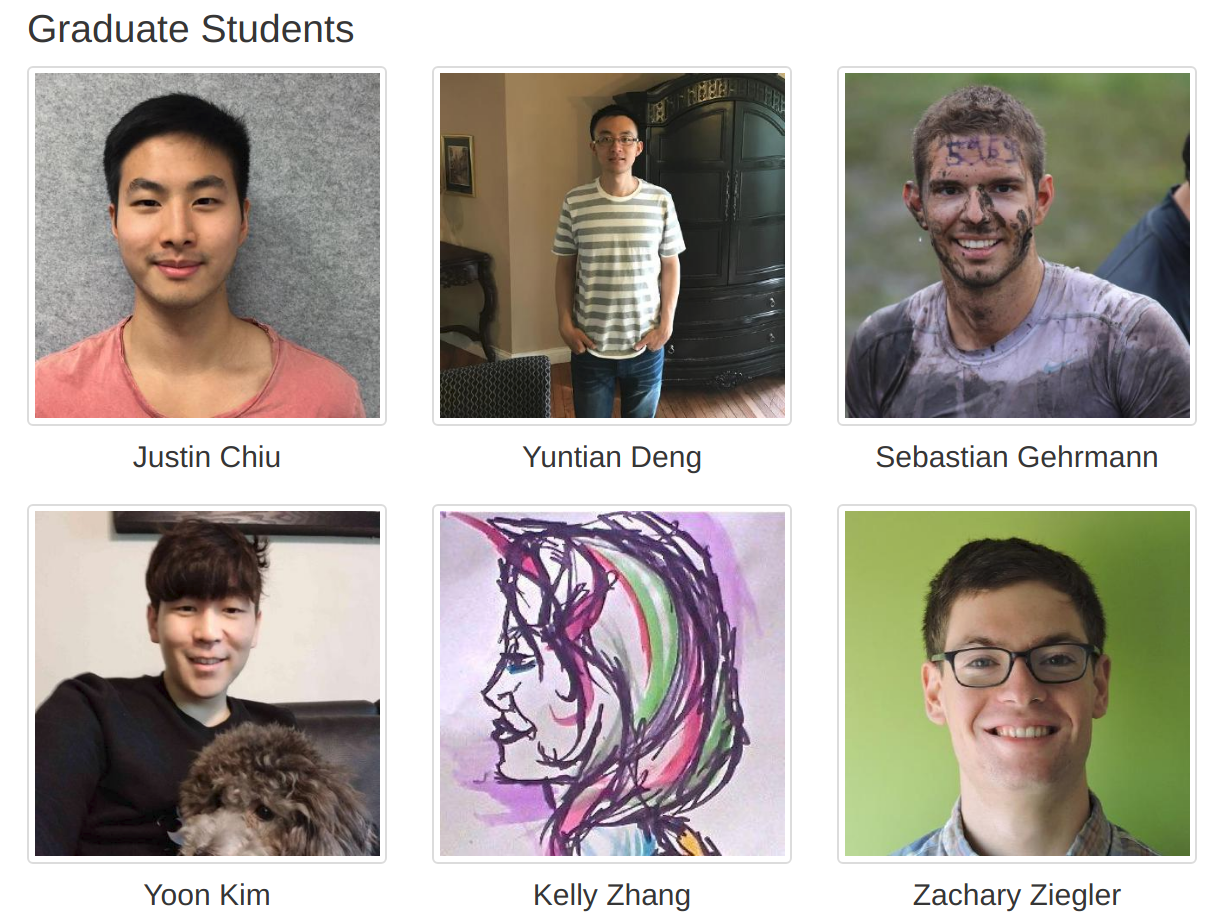
\includegraphics[width=6cm]{Members}

  
\includegraphics[width=2cm]{Members2}
  \end{center}
\end{frame}



\begin{frame}
  \url{http://lstm.seas.harvard.edu/client/lstmvis.html?project=00parens&source=states::states2&activation=0.3&cw=30&meta=..&pos=165}
  \url{http://lstm.seas.harvard.edu/client/lstmvis.html?project=05childbook&source=states::states1&activation=0.3&cw=30&meta=..&pos=100&wordBrush=..20,23&wordBrushZero=..1,0&sc=..55,59,159,167,174,179}

\end{frame}



\begin{frame}{Generation with Diagrams}
\research{\cite{Deng2016} w/ Bloomberg}
  \begin{center}
\begin{tikzpicture}


\node(a){
\includegraphics[width=1.5cm]{phone}};
 \node [yshift=4cm, rectangle, thick,fill=blue!0,text width=5cm, rounded corners, inner sep =5pt, minimum height=1em]{\baselineskip=50pt 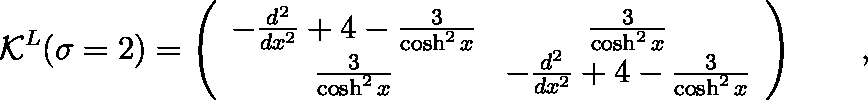
\includegraphics[width=10cm]{latexin}};

\visible {
\node (b)[xshift=6cm, rectangle, scale=0.6, draw,thick,fill=blue!0,text width=32em, rounded corners, inner sep =5pt, minimum height=1em]{\baselineskip=50pt \footnotesize
\sTWO

};
  \path[draw, <-] (b) --  (b -| gal.east);
}
\end{tikzpicture}
  \end{center}
\end{frame}


\begin{frame}{Talk about the Diagrams}
\research{\cite{Deng2016} w/ Bloomberg}
  \begin{center}
\begin{tikzpicture}


\node(a){
\includegraphics[width=1.5cm]{phone}};
 \node [yshift=4cm, rectangle, thick,fill=blue!0,text width=5cm, rounded corners, inner sep =5pt, minimum height=1em]{\baselineskip=50pt 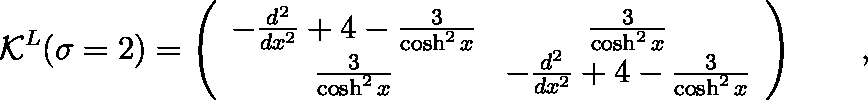
\includegraphics[width=10cm]{latexin}};

\visible {
\node (b)[xshift=6cm, rectangle, scale=0.6, draw,thick,fill=blue!0,text width=32em, rounded corners, inner sep =5pt, minimum height=1em]{\baselineskip=50pt \footnotesize
\sTWO

};
  \path[draw, <-] (b) --  (b -| gal.east);
}
\end{tikzpicture}
  \end{center}
\end{frame}

\begin{frame}
  \begin{center}
    
\includegraphics[width=0.8\textwidth]{Mathpix}
  \end{center}
\end{frame}
